\documentclass[12pt,a4paper,oneside]{article}

\usepackage{graphicx}
\usepackage{amsmath}

\begin{document}

\begin{titlepage}

\centering
	
\includegraphics[width=4cm]{logo.jpg}
	\vfill
    {\bfseries\Large
        DT2118 Lab3: Continuous Speech Recognition
        \vskip1cm
        Thomai Stathopoulou\\
        \vskip1cm
        \today
    }    
   \vfill
\end{titlepage}

\section{Training and Testing}
\subsection{Prepare the database}
After running the data preparation script, we get different files containing information about the database. That information can be summed up as follows:
\begin{itemize}
\item training set:
	\begin{itemize}
	\item 6160 male speakers (4235 men \& 1925 boys)
	\item 6389 female speakers (4388 women \& 2001 girls)
	\end{itemize}
\item testing set:
	\begin{itemize}
	\item 6236 male speakers (4311 men \& 1925 boys)
	\item 6311 female speakers (4389 women \& 1922 girls)
	\end{itemize}
\item 8623 training utterances
\item 8700 testing utterances
\item 22 phonemes (ah, ao, ay, eh, ey, f, hh, ih, iy, k, n, ow, r, s, sil, sp, t, th, uw, v, w, z)
\item 16 nodes and 36 arcs in the recognition network
\end{itemize}

\subsection{Train and test G-HMMs with different features} \label{sec:ghmm}
Looking at the configuration files provided for the features and the HMM models we can see that the MFCC features (and their variations) are all created with the same parameters that we used in Lab 1. So their configuration files are identical, except for the field \texttt{TARGETKIND}, which denotes the different feature kinds that we want to produce (MFCC, MFCC plus zeroth coefficient, etc.).

The configuration files for the HMM models, describe models of the same basic structure, i.e. all models have five states, of which only three are emitting. Additionally the transition probabilities of the states for every model are the same and the probability distributions for the different observations of every model are also identical. The characteristic that changes is the number of observations. This is a direct result of the feature kind, which every HMM model uses. The number of the features that every feature kind produces, is the number of different observations that every HMM model is expected to observe, hence the different features kinds have the following numbers of features:
\begin{description}
\item[\texttt{MFCC}] 12 features
\item[\texttt{MFCC\_0}] 13 features
\item[\texttt{MFCC\_0\_D}] 26 features
\item[\texttt{MFCC\_0\_D\_A}] 39 features
\item[\texttt{MFCC\_0\_D\_A\_Z}] 39 features
\end{description}
As already mentioned, the basic structure of the HMM models is the same for all the models. So, the number of their parameters is: $5 states + 5\times5 transitionProbabilities = 30freeParameters$. This number, however is calculated without accounting for the different constraints (eg. some of the states are not emitting and some transition probabilities are zero), which would result in a decrease of the parameters.

At the training of the HMM model, the prototype models defined in the configuration files are used. In this step we are more interested in the topology of the models and not the actual parameters. We want to create a three state HMM for every phone, so in \texttt{hmm0} we merely place the prototype models for every phone (including ``sil'' for silence). For this, a set of the training data has been scanned and the means and variances have been replaced by the global speech means and variances.

Having created the prototype model, it is trained with the training data, in order to acquire the correct means and variances. This training procedure is repeated recursively, in order for the models to be re-trained and their parameters re-estimated. This results in models \texttt{hmm1} - \texttt{hmm3} (\texttt{hmm3} contains the final set of initialised monophone HMMs).

In order to make the models more robust, we want to include to ``short pause'' (``sp'') in the training. So we create an extra model just for the short pause with only one state. This model is then connected to the ``sil'' model. The prototype for this set of models is included in \texttt{hmm4}, which then is processed in order for new transition probabilities to be added for the new states (\texttt{hmm5}). 

After this new addition, the new models are re-trained two more times, giving us \texttt{hmm6} and \texttt{hmm7}.

The models now are ready to be tested on the testing set. We can observe that for the different feature kinds we get different results. The results are summarized in Table \ref{tab:results1}.

\begin{table}
\caption{Word accuracy and correct words for different feature kinds} \label{tab:results1}
    \begin{tabular}{|c||c||c|}
    \hline
    Feature Kind                 & Correct Words / All Words (\%)   & Accuracy (Insertions) 			\\ \hline \hline
    \texttt{MFCC}                & 26392 / 28583 (92.33\%)          & 91.2 (324)           			\\ \hline
    \texttt{MFCC\_0}             & 26733 / 28583 (93.53\%)          & 92.71 (235)           			\\ \hline
    \textbf{\texttt{MFCC\_0\_D}} & \textbf{27923 / 28583 (97.69\%)} & \textbf{96.34 (385)}           \\ \hline
    \texttt{MFCC\_0\_D\_A}       & 27789 / 28583 (97.22\%)          & 93.69 (1010)                   \\ \hline
    \texttt{MFCC\_0\_D\_A\_Z}    & 27706 / 28583 (96.93\%)          & 92.44 (1285)          			\\ \hline
    \end{tabular}
\end{table}

It is obvious from this Table, that \texttt{MFCC\_0\_D} gives the best results in terms of correct words and word accuracy (97.69\% and 96.34\% respectively). \texttt{MFCC\_0\_D\_A} and \texttt{MFCC\_0\_D\_A\_Z} are quite close in terms of correct words, but have lower accuracy, since they have almost three to four times the insertion errors. \texttt{MFCC} and \texttt{MFCC\_0} have the least correct words, but their accuracies are the ones that are closest to the correct word percentage, since they have fewer insertion errors.

\subsection{Train and test GMM-HMMs with increasing number of Gaussians}
We now train GMM-HMM models with different numbers of Gaussian components per state. The results can be seen in Table \ref{tab:results2}. It is very obvious that the more Gaussian components are used, the better the performance of the model. Both accuracy and correct words percentage increase.

\begin{table} 
\caption{Word accuracy and correct words for different numbers of Gaussian components per state, using feature \texttt{MFCC\_0\_D\_A} } \label{tab:results2}
    \begin{tabular}{|c|c|c|}
    \hline
    No. of Gaussians & Correct Words / All Words (\%) & Accuracy (Insertions) \\ \hline
    2                & 28141 / 28583 (98.45\%)        & 96.37 (595)           \\ \hline
    4                & 28304 / 28583 (99.02\%)        & 97.68 (384)           \\ \hline
    8                & 28411 / 28583 (99.4\%)         & 98.31 (311)           \\ \hline
    16               & 28465 / 28583 (99.59\%)        & 98.66 (265)           \\ \hline
    \end{tabular}
\end{table}

\subsection{Tune insertion penalty parameter}
Using \texttt{MFCC\_0\_D} , which had the best performance in Section \ref{sec:ghmm}, we can see that the numbers of insertions and deletions are unbalanced (385 insertions over 190 deletions - almost twice as many insertions as deletions). After running this experiment again using different Insertion Penalty parameters, we get the results shown in Table \ref{tab:penalty}. First we can observe that, the lower the penalty parameter, the higher the number of insertions occurring (as would be expected). So as we increase the penalty parameter, the insertions decrease and the deletions increase. Additionally we observe an slight increase in the system's accuracy and a similar decrease int the number of correct words. The closest to a balance we achieve with a penalty parameter 30.0.

\begin{table}
\caption{Influence of the Insertion Penalty Parameter on the performance of the models} \label{tab:penalty}
    \begin{tabular}{|c|c|c|c|c|}
    \hline 
    Penalty Parameter & Insertions   & Deletions    & Correct Words & Accuracy \\ \hline \hline
    10.0              & 602          & 154          & 97.79\%          & 95.69\%  		  \\ \hline
    20.0              & 385          & 190          & 97.69\%          & 96.34\%  		  \\ \hline
    25.0              & 290          & 228          & 97.51\%          & 96.5\%   		  \\ \hline
    \textbf{30.0}     & \textbf{241} & \textbf{257} & \textbf{97.38\%} & \textbf{96.54\%}  \\ \hline
    40.0              & 156          & 320          & 97.15\%          & 96.61\%  		  \\ \hline
    \end{tabular}
\end{table}

\subsection{Forced Alignment}
After using Wavesurfer to check the alignment between the phonemes and the actual sounds, we can conclude that the alignment is quite good. There are, of course some misalignments, that are observed by the naked eye, but in general it seems to be a good correspondence between sounds and phonemes.

\section{Analysis}

\subsection{Parameter evolution at different iterations}
Figures \ref{fig:means} and \ref{fig:variances} show the evolution of the means and variances along the iterations respectively. The chosen model implements the phoneme ``r'' and the chosen state is the second. We can see that the means start at a value close to zero, except for the mean of the zeroth coefficient, which starts off at a higher value. They need 2-3 iterations in order to settle to an almost constant value. The is a slight change in the values at the fifth iteration, but in most case the change is almost negligible.

The variances, on the other hand start of at much higher values. Even though they are more spread out, still most of them seem to be closer together, having the zeroth coefficient as an outlier. In the first three iterations we can observe a big change in all the values. After the third iteration the variances seem to behave similarly to the means. So depending on how much steadiness we need for our parameters, we could stop the training at the third iteration, or let it train more, in order to check weather it becomes more steady.

\begin{figure}[h]
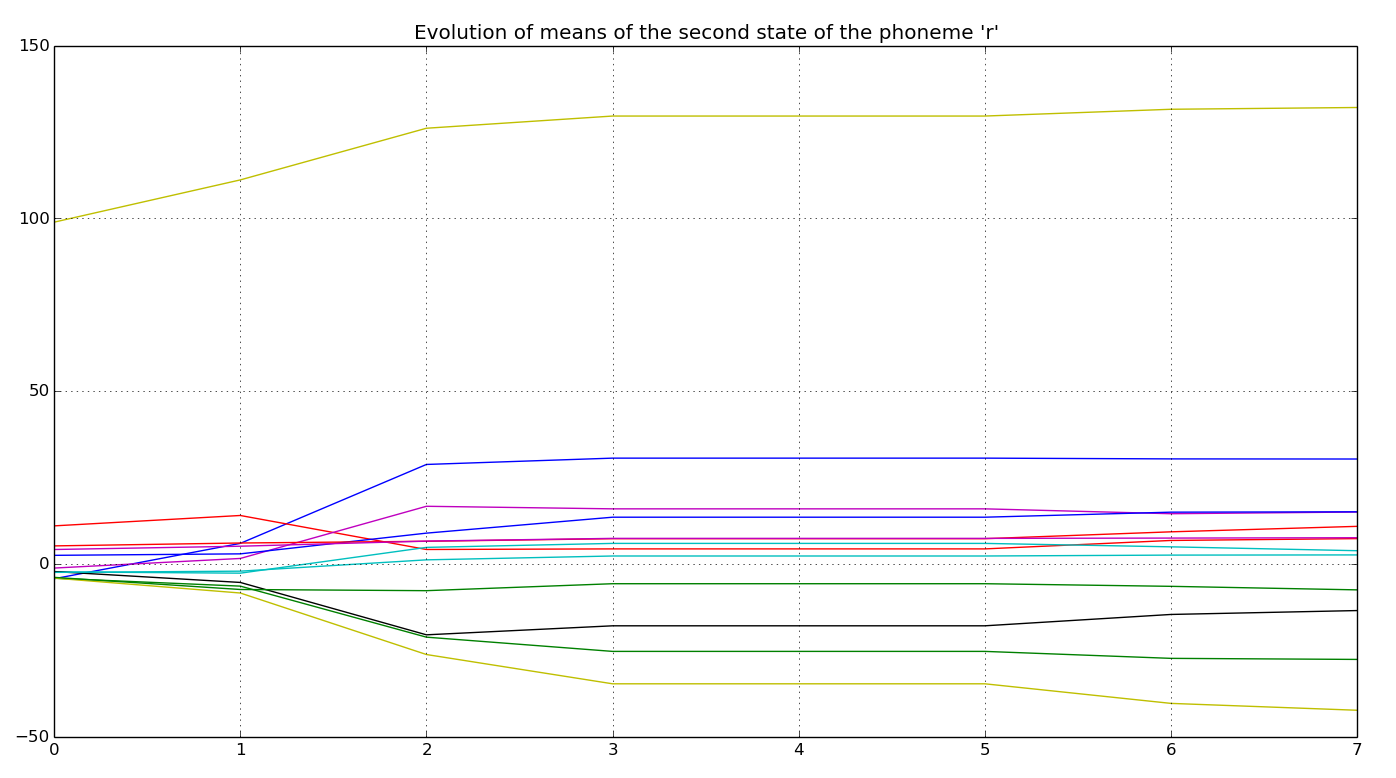
\includegraphics[scale=0.4]{means.png}
\caption{Evolution of means of the second state of the phoneme ``r''}
\label{fig:means}
\end{figure}

\begin{figure}[h]
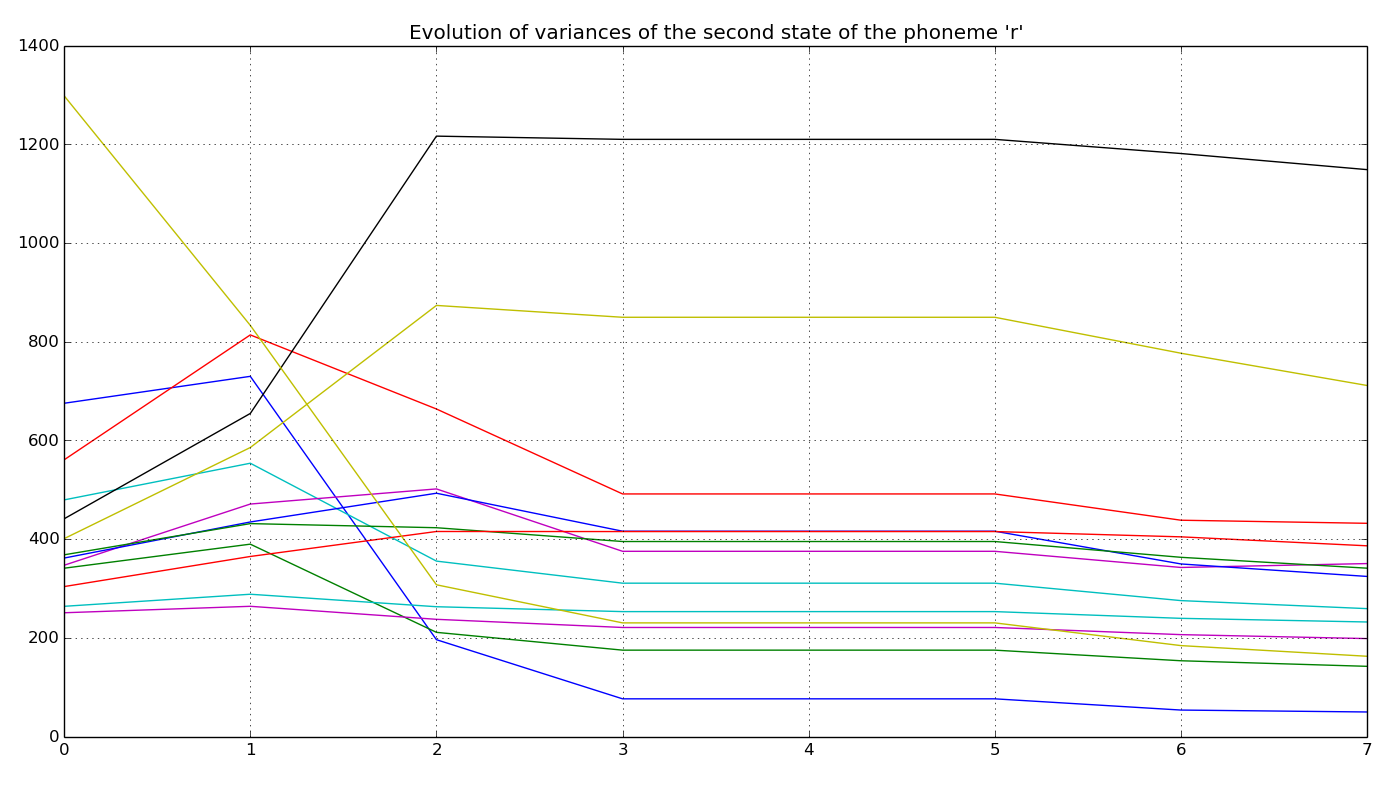
\includegraphics[scale=0.4]{variances.png}
\caption{Evolution of variances of the second state of the phoneme ``r''}
\label{fig:variances}
\end{figure}



\subsection{Parameters for different phonemes}
For the last task of the Lab, we plot the means (MFCC features) of different phonemes. These features can be seen in Figure \ref{fig:mfccs}. First we can observe that this Figure is in accordance with the means' behaviour in Figure \ref{fig:means}. We can see that in the last iteration of Figure \ref{fig:means}, the zeroth coefficient has a much higher value than the rest (similar to the start off values), which have values around zero.

Now, in Figure \ref{fig:mfccs} we can see a similar behaviour. The zeroth coefficient of all three MFCC features has a high value, whereas the rest of the coefficients are all closer to zero. Of course there is an obvious difference between the ``patterns'' of the graphs between different phonemes. The graph representing the MFCC of ``sil'', has a very low variance and remains almost steadily close to zero (an expected behaviour for this particular phoneme). On the contrary, the behaviour of ``ao''  has much larger differences between different coefficients. Finally the graph representing ``s'', lies somewhere in the middle of the other two. It is not as steady as the ``sound of silence'', but is much steadier that the sound of a vowel (``ao'').

These difference are much more visible in Figure \ref{fig:inv_dcts}, where we see the phonemes' features one step before their final form (which is used for the recognition and classification). Here the behaviours of the graphs, as described in the previous paragraph are more obvious, proving that these feature are indeed indicative of the phoneme that produced them. 

\begin{figure}
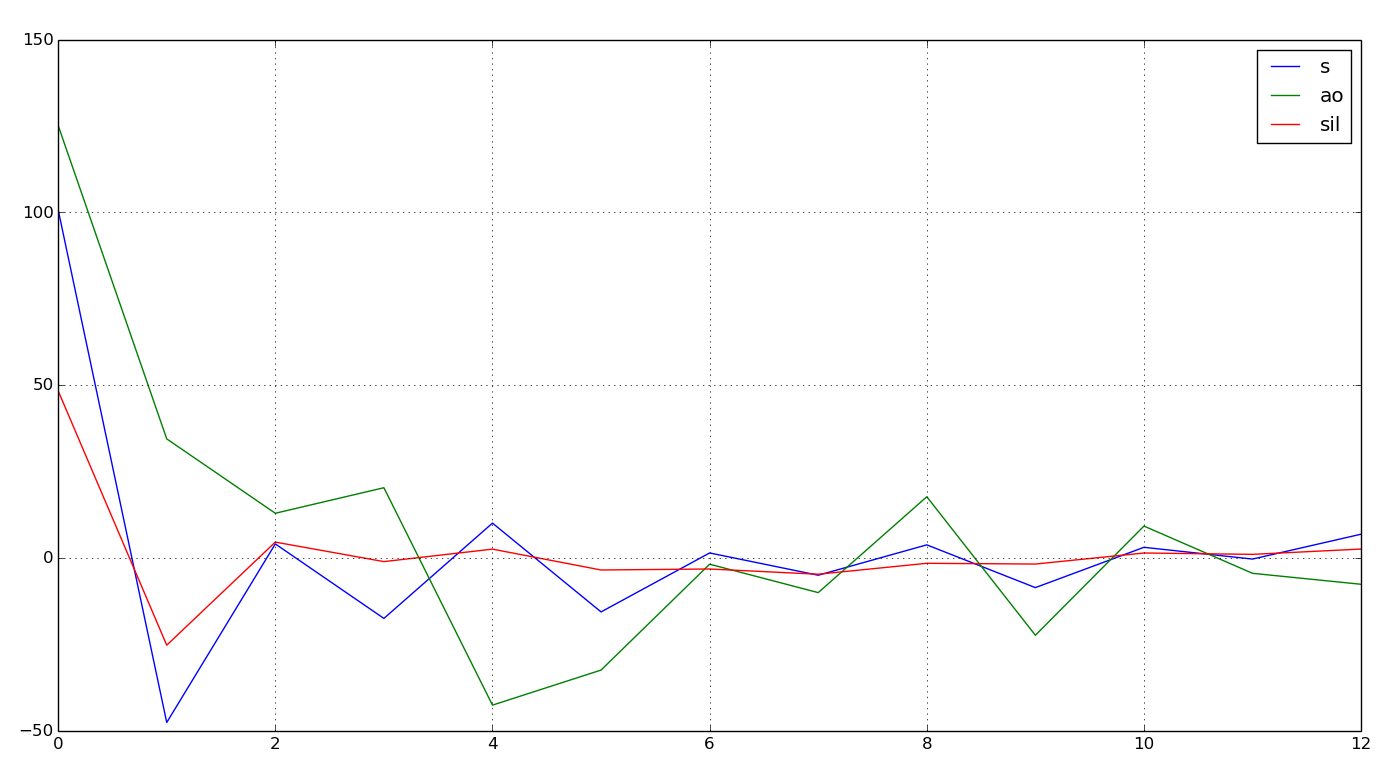
\includegraphics[scale=0.4]{mfccs.png}
\caption{MFCC features for different phonemes}
\label{fig:mfccs}
\end{figure}

\begin{figure}
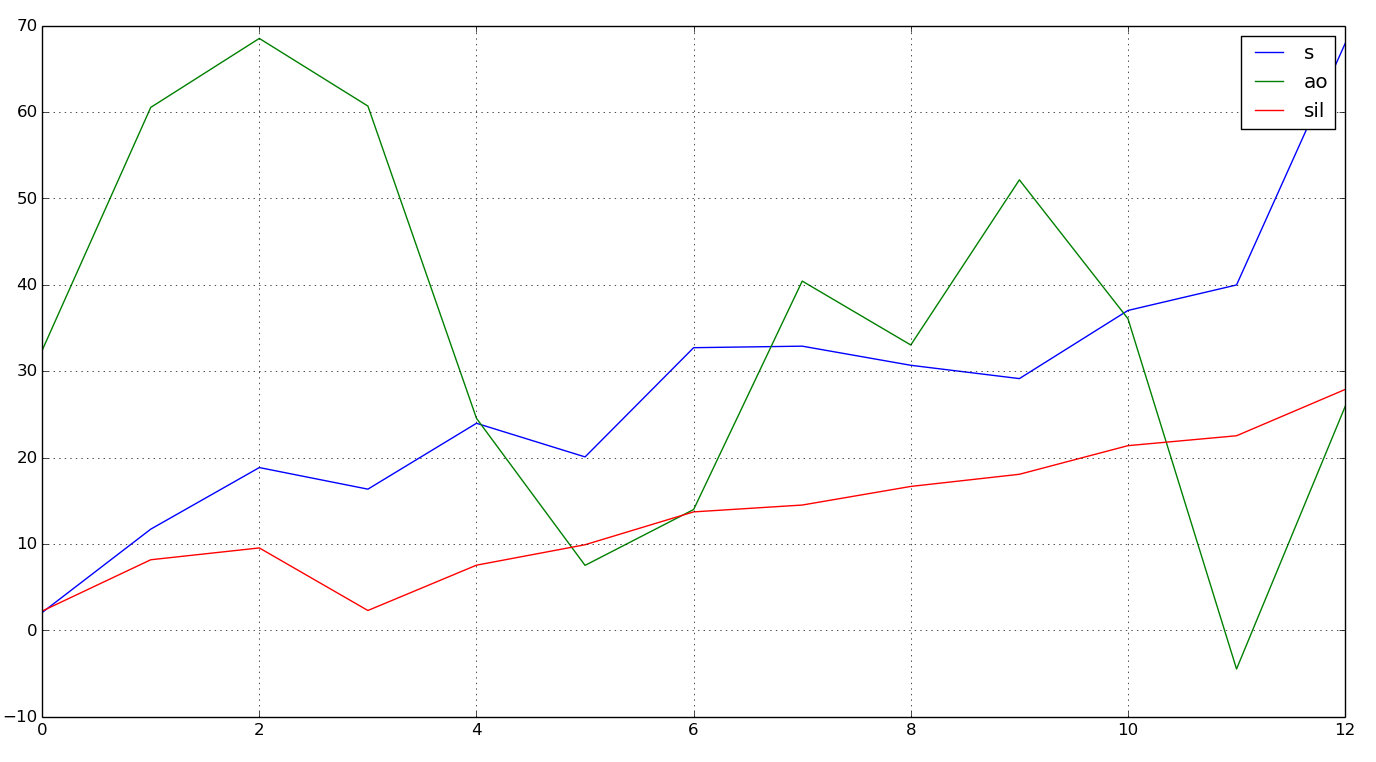
\includegraphics[scale=0.4]{inverse_dct.png}
\caption{Filterbank outputs of features for different phonemes}
\label{fig:inv_dcts}
\end{figure}





\end{document}